\documentclass[a4paper,12pt]{article}

\usepackage[utf8]{inputenc}
\usepackage{amsmath, amssymb}
\usepackage{graphicx}
\usepackage{caption}
\usepackage{tcolorbox}
\usepackage{geometry}
\geometry{margin=1in}

\title{\textbf{Statistical Report: Law of Large Numbers and Central Limit Theorem}}
\author{}
\date{}

\begin{document}

\maketitle

% ---------------- INTRO ----------------
\section{Introduction}

Statistics is built on two fundamental pillars: the Law of Large Numbers (LLN) and the Central Limit Theorem (CLT). These results explain why randomness becomes predictable at scale and why the normal distribution appears everywhere in data science, physics, and machine learning.

This report explores their meaning, intuition, and practical behavior using simulations and examples.

% ---------------- LLN ----------------
\section{Law of Large Numbers (LLN)}

\subsection{Mathematical Statement}

\[
\bar{X}_n \rightarrow \mathbb{E}[X] \quad \text{as } n \to \infty
\]

\subsection{Intuition}

\begin{tcolorbox}
The more observations you take, the closer your average gets to the true expected value.
\end{tcolorbox}

Early results can fluctuate heavily, but randomness “averages out” over time.

\subsection{Concrete Examples}

\textbf{Example 1: Coin Toss}
\begin{itemize}
\item Let heads = 1, tails = 0
\item Expected value = 0.5
\item After 10 tosses → unstable average
\item After 10,000 tosses → converges to 0.5
\end{itemize}

\textbf{Example 2: Dice Roll}
\begin{itemize}
\item Expected value = 3.5
\item Small samples fluctuate
\item Large samples stabilize around 3.5
\end{itemize}

\subsection{Interpretation}

The LLN does NOT say results become identical — it says the \textbf{average becomes stable}. This is why averages in real datasets are meaningful.

% ---------------- CLT ----------------
\section{Central Limit Theorem (CLT)}

\subsection{Mathematical Statement}

\[
\frac{\bar{X} - \mu}{\sigma / \sqrt{n}} \rightarrow \mathcal{N}(0,1)
\]

\subsection{Intuition}

\begin{tcolorbox}
No matter the original distribution, the distribution of sample means becomes approximately normal when $n$ is large.
\end{tcolorbox}

This is one of the most powerful results in statistics.

\subsection{Concrete Examples}

\textbf{Example 1: Exponential Data}
\begin{itemize}
\item Original data is highly skewed
\item Sample means become symmetric as $n$ increases
\end{itemize}

\textbf{Example 2: Uniform Distribution}
\begin{itemize}
\item Flat distribution initially
\item Sample means form a bell curve
\end{itemize}

\textbf{Example 3: Bernoulli Trials}
\begin{itemize}
\item Individual outcomes are binary
\item Means converge to a normal shape
\end{itemize}

\subsection{Why variance decreases}

\[
\text{Var}(\bar{X}) = \frac{\sigma^2}{n}
\]

As $n$ increases:
\begin{itemize}
\item spread decreases
\item estimates become more precise
\item curve becomes sharper around $\mu$
\end{itemize}

% ---------------- INTERPRETATION ----------------
\section{Interpretation and Key Insights}

\begin{tcolorbox}
\textbf{LLN = stability of the mean} \\
\textbf{CLT = shape of the distribution of the mean}
\end{tcolorbox}

\subsection{Interpretation of the Law of Large Numbers}

The LLN figure illustrates the evolution of the cumulative mean as the number of observations increases. At small sample sizes, the mean fluctuates significantly due to randomness. However, as the number of observations grows, these fluctuations decrease and the mean stabilizes around the theoretical expected value.

This convergence is not smooth but oscillatory, meaning the sample mean continues to vary but within a progressively smaller range. This demonstrates that large samples provide more reliable and stable estimates.

\subsection{Interpretation of the Central Limit Theorem}

The histograms show the distribution of sample means for different underlying distributions (uniform, exponential, and Bernoulli). For small sample sizes, the shape of the distribution reflects the original data. As the sample size increases, the distributions become more symmetric and gradually resemble a bell-shaped curve.

This confirms that regardless of the initial distribution, the distribution of sample means converges toward a normal distribution, which is the essence of the Central Limit Theorem.

\subsection{Q-Q Plot Analysis}

The Q-Q plot compares the quantiles of the sample means to those of a theoretical normal distribution. While the central points are approximately aligned along the diagonal, noticeable deviations appear in the tails.

This indicates that the distribution of sample means is approaching normality but has not fully converged. Such deviations are expected when the sample size is not sufficiently large or when the original distribution is strongly skewed (as in the exponential case).

\subsection{Global Insight}

Together, the results highlight two complementary phenomena:
\begin{itemize}
\item The LLN ensures that estimates become stable and converge toward the true mean.
\item The CLT explains why the distribution of these estimates tends toward a normal shape.
\end{itemize}

Thus, randomness does not disappear as more data is collected; instead, it becomes structured and predictable. This dual behavior is the foundation of statistical inference and justifies the widespread use of normal-based methods in data analysis.


% ---------------- FIGURES ----------------
\section{Figures}

\subsection{Central Limit Theorem}

\begin{figure}[h]
\centering
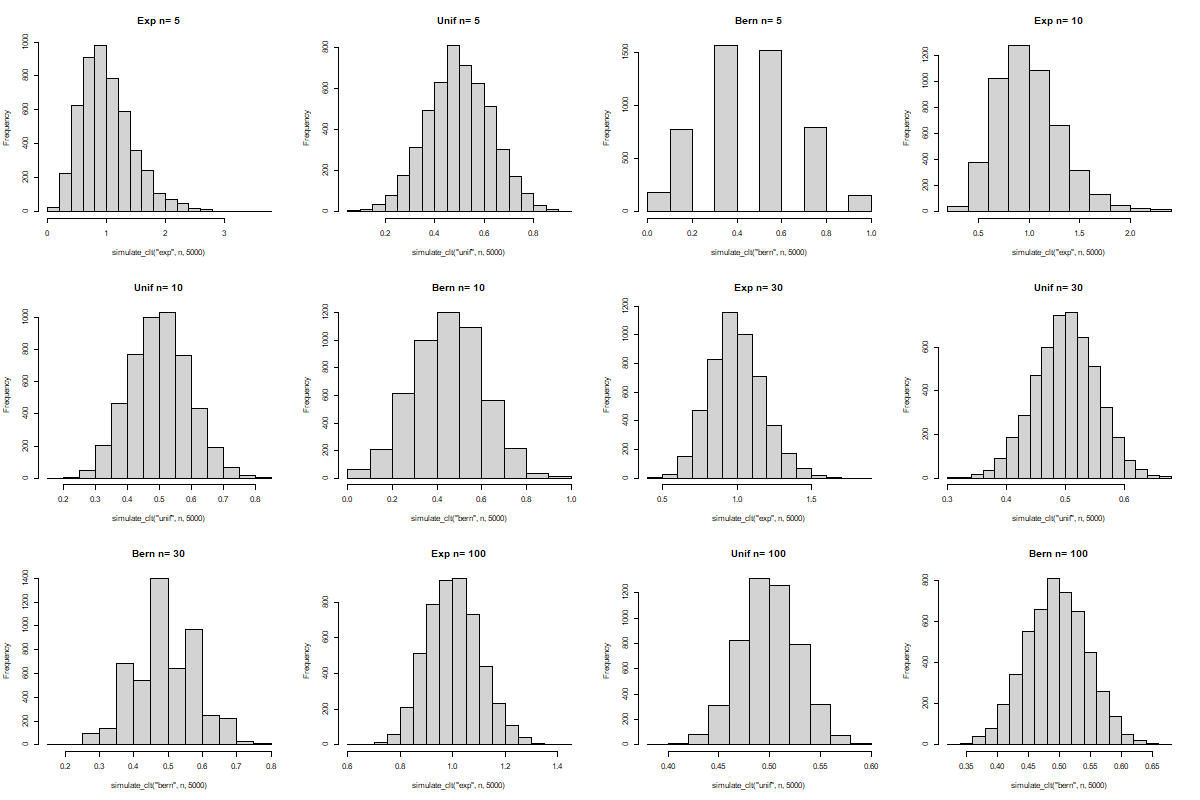
\includegraphics[width=\textwidth]{../plots/clt_comparison.png}
\caption{CLT: Distribution of sample means becomes normal as sample size increases.}
\end{figure}

\subsection{Q-Q Plot}

\begin{figure}[h]
\centering
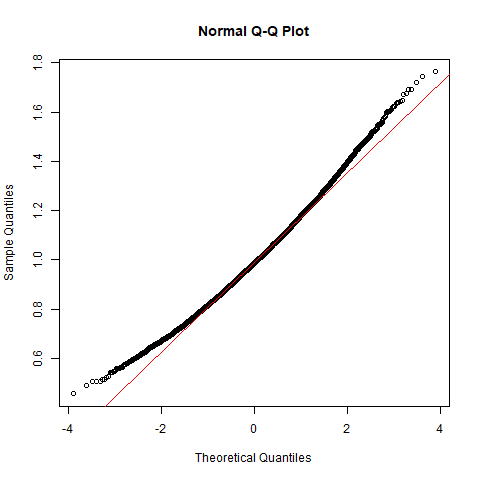
\includegraphics[width=0.6\textwidth]{../plots/clt_exp_qq.png}
\caption{Q-Q plot showing approximate normality of sample means.}
\end{figure}

\subsection{Law of Large Numbers}

\begin{figure}[h]
\centering
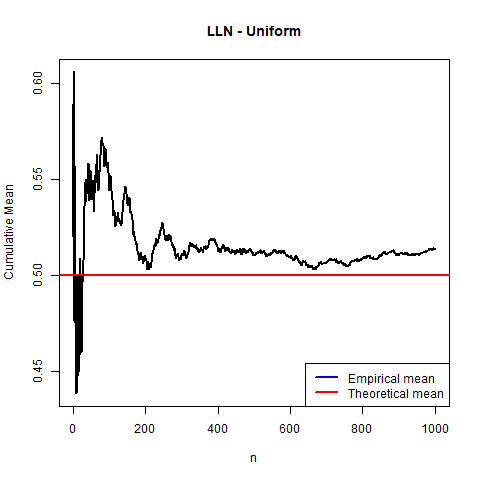
\includegraphics[width=0.6\textwidth]{../plots/lln_uniform.png}
\caption{LLN: convergence of sample mean toward expected value.}
\end{figure}

% ---------------- CONCLUSION ----------------
\section{Conclusion}

The Law of Large Numbers ensures that averages become stable with large samples, while the Central Limit Theorem explains why these averages follow a normal distribution.

Together, they form the foundation of statistical reasoning, enabling prediction, estimation, and hypothesis testing across data science and real-world applications.

\end{document}
